\chapter{Perancangan}
\label{chap:design}

Pada bab ini akan dipaparkan berbagai macam rancangan dari perkakas \cl yang akan dibuat, seperti diagram-diagram terkait, masukan serta keluaran perangkat lunak,
% Jangan lupa - bagian ini belum selesai!

\section{Diagram}
\label{sec:analysis-diagrams}

Bagian ini akan membahas mengenai alur dari \textit{activity diagram} serta \textit{sequence diagram} dari perkakas yang akan dibuat.
% Tambahkan deskripsi jika diagram kelas tidak dibuat!!

\section{\textit{Activity Diagram}}
\label{sec:design-diagrams-activity}

Ada tiga buah \textit{activity diagram} dari perkakas ini, di mana masing-masing diagram merepresentasikan tiap-tiap fitur yang akan diimplementasikan. Adapun 
% Belum selesai!

\begin{figure}[ht]
    \centering
    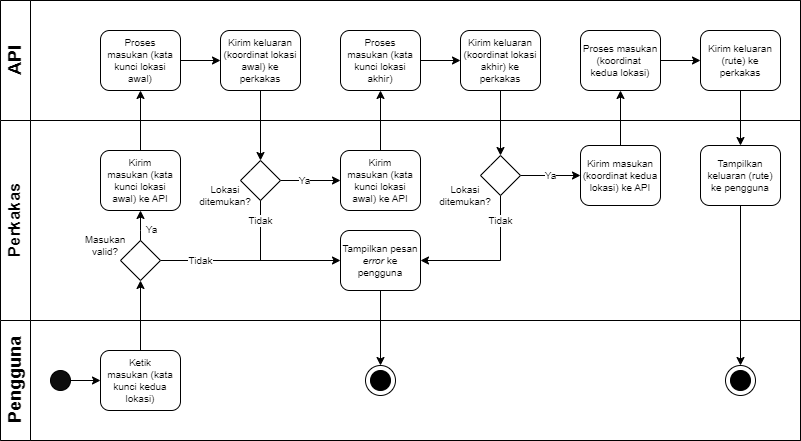
\includegraphics[width=\linewidth]{diagrams-activity-direct}
    \caption[Diagram \textit{use case} perkakas yang akan dibangun]{Diagram \textit{use case} dari perkakas yang akan dibangun.}
    \label{fig:diagrams-activity-direct}
\end{figure}

\section{\textit{Sequence Diagram}}
\label{sec:design-diagrams-sequence}
